\documentclass[10pt,letterpaper]{article}
\usepackage[margin=0.88in]{geometry}
\usepackage[T1]{fontenc}
\usepackage[utf8]{inputenc}
\usepackage{lmodern,microtype,amsmath,amssymb,amsthm,mathtools}
\usepackage{booktabs,longtable,array,tabularx,enumitem,xcolor}
\usepackage{tikz}
\usetikzlibrary{arrows.meta,positioning}
\usepackage{xurl,hyperref,fancyhdr}
\definecolor{ink}{HTML}{18354A}
\definecolor{accent}{HTML}{176E78}
\hypersetup{colorlinks=true,linkcolor=ink,urlcolor=accent,citecolor=ink,pdftitle={New 194-state PA-consistency machines by changing the constructor coefficient},pdfauthor={Research prepared for Vladimir Reshetnikov}}
\pagestyle{fancy}\fancyhf{}\fancyhead[L]{\small PA consistency machines: constructor coefficients 5 and 6}\fancyhead[R]{\small 13 November 2026}\fancyfoot[C]{\thepage}
\setlength{\headheight}{14pt}
\setlength{\parskip}{4pt}\setlength{\parindent}{0pt}
\setlist{nosep,leftmargin=1.6em}
\newtheorem{theorem}{Theorem}
\newtheorem{lemma}[theorem]{Lemma}
\newtheorem{proposition}[theorem]{Proposition}
\newcommand{\PA}{\mathsf{PA}}
\newcommand{\Con}{\operatorname{Con}}
\newcommand{\Halt}{\operatorname{Halt}}
\newcommand{\Prf}{\operatorname{Prf}}
\newcommand{\Bit}{\operatorname{Bit}}
\newcommand{\pair}{\mathsf p}
\newcommand{\file}[1]{\nolinkurl{#1}}
\newcommand{\act}[3]{#1\,\mathrm{#2}\,#3}
\title{\color{ink}New 194-state PA-consistency machines\\[4pt]\large Constructor coefficients 5 and 6, a shared decoder, and a complete corpus comparison}
\author{Research prepared for Vladimir Reshetnikov}
\date{13 November 2026, Pacific time}
\begin{document}
\maketitle
\begin{abstract}
No verified machine with fewer than 194 working states was obtained. The requested alternative is supplied by two new, complete, blank-start binary Turing machines, $M_5$ and $M_6$, with 194 working states each. They use the numerical formula constructors $k\pair(a,b)+r$, with $k=5,6$ and tags $r=0,1,2,3$, in place of the previous coefficient four. A restructuring of the multiplication decoder makes its two-increment subroutine reachable only after a written one. That context permits a three-transition implementation shared with a different control reached after a written zero. The count is $135+67-8=194$.

The new arithmetic encoding is calibrated to PA by an injective hereditary recoding of both formula codes and variable labels. Its failure to preserve numerical order is handled using the already proved unrestricted dominated-implication theorem. Independent literal-tape checks cover every primitive source outcome, derive the four register-list lemmas from the actual rows, and verify the complete blank startup. A third 194-state machine, $M_{4R}$, applies the new decoder mechanism while preserving the original resolved source graph exactly. The results are ordinary mathematical PA-provability arguments with executable certificates; they are not newly compiled end-to-end Lean or Rocq theorems.
\end{abstract}
\tableofcontents

\section{Result, conventions, and exact scope}

Every delivered main table has alphabet $\{0,1\}$, one two-way infinite tape, and an all-zero initial tape. Every transition writes one bit and moves exactly one cell left or right. Working states exclude the terminal halt label. In the dense tables the working labels are $0,\ldots,193$, the start is $0$, and the halt label is $194$. There are exactly 388 transition rows and no outgoing row at halt.

\begin{theorem}[New constructor-coefficient machines]
For each $k\in\{5,6\}$, the literal table $M_k$ supplied with this report satisfies
\[
  \PA\vdash\bigl(\neg\Halt(M_k,\text{blank})\ \longleftrightarrow\ \Con(\PA)\bigr).
\]
The new 194-state companion $M_{4R}$ satisfies the same statement and has a PA-formalizable blank-halting equivalence with the pinned primary PA194 table.
\end{theorem}

Here $\Con(\PA)$ is the absence of a finite proof of $0=1$ in a fixed ordinary recursively checked first-order PA proof system. The theorem concerns an arithmetized finite run of the exact transition table, not just its execution over the standard natural numbers. The proof combines the source-calculus translation in Section~\ref{sec:logic}, the exact source binding, and the universal physical simulation. Its inherited PA-refutation compiler and diagonal-calibration interfaces are identified explicitly below.

The construction fulfills the alternative 194-state target. It does not lower the current count and does not claim faster proof search. In fact the coefficient-5 and coefficient-6 programs contain more primitive increment sites, and the larger numerical codes can increase running time. Their value is a different arithmetic encoding with a fully specified state allocation and a new family for subsequent optimization.

\begin{center}\small
\begin{tabular}{@{}lll@{}}
\toprule
Machine & Construction & Dense-table SHA-256 \\\midrule
$M_{4R}$ & Source-preserving reassociation & \begin{tabular}[t]{@{}l@{}}\ttfamily a3c1d556d61b37d60639801accacfa59\\\ttfamily 5df4b2c9d2b2a0a46978425b10c459a8\end{tabular}\\[4pt]
$M_5$ & Constructor coefficient 5 & \begin{tabular}[t]{@{}l@{}}\ttfamily 180a0fd1f046d4cbd687b43979f06056\\\ttfamily 19ad5f53054d32b9f62f33e7a3bccab8\end{tabular}\\[4pt]
$M_6$ & Constructor coefficient 6 & \begin{tabular}[t]{@{}l@{}}\ttfamily 725ce8474d7b83473488fc9466548ed2\\\ttfamily de3744d9a80183467894f9d719103ab2\end{tabular}\\[4pt]
\bottomrule\end{tabular}
\end{center}


\section{Comparison of the requested corpus}
\label{sec:corpus}

The comparison is pinned to ProveIt commit
\begin{center}\small\texttt{17f92105e2bc4317feae6c219cb2143437b482ff}.\end{center}
The requested PA directory and incoming archives were inspected, together with relevant ZFC and ConciseIPRA material. The corpus includes 36 packets already placed under \file{PA/docs} and five newer packets: 41 delivered packet families. Twenty-six ZIP files remain directly under \file{docs/incoming}; 21 of these overlap the placed collection. The complete packet ledger appears in Appendix~\ref{app:ledger} and in machine-readable form.

The table recognizer found 4,421 occurrences of complete numeric five-column tables, representing 621 distinct byte forms, in direct files and 44 distinct ZIP payloads referenced 71 times. There were no unread or skipped archives. It found no recognized table with 10 through 193 working states. Small synthetic examples and rejected experiments were retained in the inventory rather than counted as consistency machines. Tables encoded only in arbitrary source code, JSON, or prose are outside this literal-table recognizer's scope; the packet narratives were read separately. This census is not a proof that no smaller design exists.

The critical 194-state comparison is broader than the main report files alone:

\begin{center}\small
\begin{tabularx}{\linewidth}{@{}lX@{}}
\toprule
Existing class & Distinguishing feature and status \\
\midrule
Primary PA194 & $134+67-7$; 3,673 source sites; separated diagonal head. \\
PA194\_AD & Same source, different physical A/D register placement. \\
Eight-fold PA194 & $134+68-8$; alternative AX decoder allocation. \\
Rejected scanner quotient & A source address violates the return-scanner contract; not an accepted consistency construction. \\
PA194C & Cached combined controller; 3,649 sites. Several later packets repeat exactly the same primary table. \\
PA194CS & Symmetric destructive-equality implementation of Shift; 3,646 sites. \\
PA194altC & Auxiliary combination of the cached controller and eight-fold decoder. \\
PA194CZ & Auxiliary known-zero conditional-decrement implementation of a source jump. \\
\bottomrule
\end{tabularx}
\end{center}

These eight graph classes occur as 15 table byte forms, including native/dense relabelings. At 195 states the recognizer finds 26 byte forms in 16 graph classes; at 196 states, 163 forms in 99 classes. Those counts include rejected and diagnostic objects.

The larger families establish the ancestry and explain why apparently independent savings often do not add. The U208 lineage compresses an older PA checker using contextual folds, frame-aware source simulations, register placement, and source rotations. James Chang's PA209/PA196 lineage changes the logical interface and constructor layout; the imported PA196 development supplies the internal PA-refutation-to-halting direction. The subsequent diagonal 195-state designs replace a larger equality-vacuity component by code-driven diagonal vacuity. Separating that diagonal clause into its own pushed stack head shortens the AX emitter to 190 macro tokens. The first primary 194-state design then combines 67 raw readers with seven compatible folds. Cached-controller and symmetric-Shift variants modify the fixed program instead. The new work changes the constructor multiplier and its fixed decoder, while retaining the separated-head logical interface.

The novelty comparison canonicalizes the new complete transition graphs against all prior 194-state tables, allowing arbitrary control renaming, arbitrary choice of a root reaching the whole graph, global left/right reflection, and global read/write-bit complementation. $M_5$, $M_6$, and $M_{4R}$ are pairwise distinct and absent from the old classes even under this deliberately stronger comparison. Bit complementation is used only as an exclusion test; the delivered machines still start on zero tape.

\section{Changing the constructor coefficient}
\label{sec:constructor}

Write Cantor pairing as
\[
 \pair(a,b)=\frac{(a+b)(a+b+1)}2+b.
\]
For a fixed $k\ge4$, define the numerical constructors
\begin{align*}
 I_k(A,B)&=k\pair(A,B), & M_k(a,b)&=k\pair(a,b)+1,\\
 U_k(a,B)&=k\pair(B,a)+2, & E_k(a,b)&=k\pair(a,b)+3.
\end{align*}
The transposition in $U_k$ is intentional. In this section $M_k(a,b)$ denotes a formula constructor, while the standalone symbol $M_k$ denotes the delivered machine; the arguments distinguish them. Code zero is truth, code one is $M_k(0,0)$ and is the designated contradiction, and $N_k(B)=I_k(B,1)$ is negation. Conjunction and existential quantification are the usual classical implicational abbreviations.

For $k>4$, some residues are unused. In the PA interpretation they decode as truth. This supplies a total interpretation of every natural number, including every possible arithmetic parameter encountered by the checker. It does not add an axiom saying that each unused number is a theorem of the searched calculus.

\subsection{The exact source change}

The source register order is $(N,T,W,A,D,H,X,Y,L)$. Thus $T$ is register 1 and $Y$ is register 7. The original constructor macro \file{node65} computes a stack operation with the effect
\[
 (T,W)=(a,\pair(b,w))\ \longmapsto\ (k\pair(b,a),w),
\]
when entered with $X=Y=0$; it restores $X=Y=0$ and preserves every other register. Its unchanged prefix decodes the stack head and computes the Cantor pair. The final loop consumes $Y$ and increments $T$ a fixed number of times for each consumed unit.

In the old source \file{node61} is four consecutive increments of register 1. It is used only by \file{node62}, the per-unit body of this constructor loop. The new source replaces it with five or six consecutive increments. The explicit source binding checks 61 expanded occurrences, all 61 surrounding constructor prefixes, every loop test and back edge, all 3,429 primitive sites outside these bodies, and every outside successor under the index relocation. No source edge enters the interior of a replacement body from outside it.

Consequently the complete source sizes are
\[
 3429+61\cdot4=3673,\quad
 3429+61\cdot5=3734,\quad
 3429+61\cdot6=3795.
\]
The literal tag increments after the constructor remain unchanged. The AX word still contains exactly 190 macro tokens. The same constructor is used when MP constructs the implication whose code is compared with the cached theorem; changing the emitter without changing this MP constructor would be incorrect.

\begin{lemma}[Generic constructor loop]
If the final loop begins with $T=t$ and $Y=y$, its coefficient-$k$ body terminates with $T=t+ky$ and $Y=0$, preserving all other registers.
\end{lemma}
\begin{proof}
Use the invariant $T+kY=t+ky$. A positive loop iteration decrements $Y$ once and increments $T$ exactly $k$ times, preserving the invariant; the zero branch exits. Induction on the initial $y$ gives termination and the stated result. Combining this with the unchanged stack-decoding and pairing prefix proves the macro contract above. This is a primitive-recursive finite computation with a PA proof, uniformly for each fixed $k$.
\end{proof}

This macro argument is additional to the primitive instruction certificates: implementing the changed primitive graph does not alone prove its intended constructor semantics. The archive includes the detailed source lemma and an exact free-algebra AX-emitter audit. That audit checks all ten pushed entries, the six retained axiom heads, the separated diagonal head, the guarded final top, and their ordering.

\section{The decoder allocation and the eighth fold}
\label{sec:fold}

Let $i$ denote one increment of $T$, and let $D=(i,i)$ denote the two-increment subtree. The old multiplier tree is $(D,D)$, so the physical decoder for $D$ can be entered after either bit. For the new coefficient-five tree choose $((i,D),D)$; for coefficient six choose $((i,D),(i,D))$. Now every entry into $D$ in the multiplier is a right-child entry. The existing AX uses of $D$ are also right-child entries. Therefore the cell just left of its head is always one.

\begin{center}
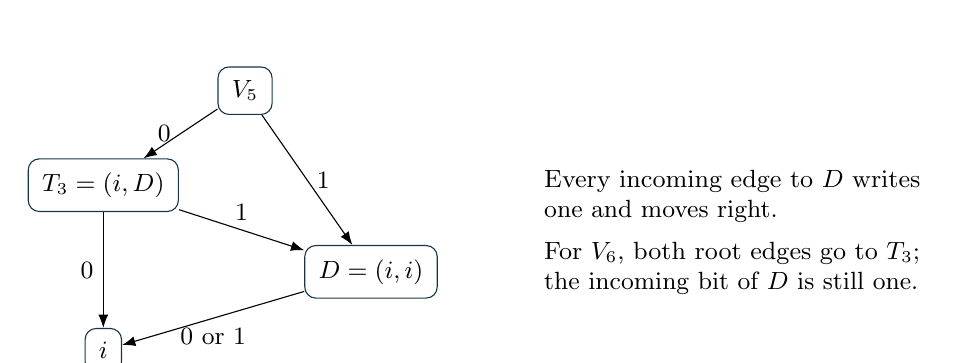
\begin{tikzpicture}[>=Latex, every node/.style={font=\small},box/.style={draw=ink,rounded corners,inner sep=5pt},x=1cm,y=1cm]
\node[box] (v) at (0,1.8) {$V_5$};
\node[box] (t) at (-1.8,0.6) {$T_3=(i,D)$};
\node[box] (d) at (1.6,-0.5) {$D=(i,i)$};
\node[box] (i) at (-1.8,-1.5) {$i$};
\draw[->] (v)--node[left] {0} (t);
\draw[->] (v)--node[right] {1} (d);
\draw[->] (t)--node[above] {1} (d);
\draw[->] (t)--node[left] {0} (i);
\draw[->] (d)--node[below] {0 or 1} (i);
\node[align=left,text width=5.0cm] at (6.3,0) {Every incoming edge to $D$ writes one and moves right.\par\vspace{4pt}For $V_6$, both root edges go to $T_3$; the incoming bit of $D$ is still one.};
\end{tikzpicture}
\end{center}

Native control 99 implements $D$. A different fixed decoder, control 41, has incoming rows only from controls 28 and 70, each writing zero and moving right. The changed multiplier therefore makes the two controls distinguishable by a tape bit already present, without adding a new tape marker.

Add control 330 with rows $\act{0}{R}{61}$ and $\act{1}{R}{99}$. In the raw table, change control 190 as follows:
\begin{center}
\begin{tabular}{@{}lcc@{}}\toprule
Family & Reading 0 at 190 & Reading 1 at 190 \\\midrule
$M_{4R}$ & $\act{0}{R}{61}$ & $\act{1}{R}{330}$ \\
$M_5$ & $\act{0}{R}{330}$ & $\act{1}{R}{99}$ \\
$M_6$ & $\act{0}{R}{330}$ & $\act{1}{R}{330}$ \\
\bottomrule\end{tabular}
\end{center}
Finally redirect control 41 to 99, delete 41, and give 99 the rows
\[
  (99,0)\mapsto\act{0}{L}{30},\qquad
  (99,1)\mapsto\act{1}{L}{2035}.
\]
The two helpers are already present. Four local cases prove the fold. In the following table $h$ is the bit immediately left of the head, $b$ is the bit being read, and the last column is the effect of the original one-step transition, reproduced by three new transitions.
\begin{center}\small
\begin{tabular}{@{}cccll@{}}\toprule
Old control & $h$ & $b$ & New control trace & Final action \\\midrule
41 & 0 & 0 & $99,30,45,24$ & $\act{0}{R}{24}$ \\
41 & 0 & 1 & $99,2035,61,25$ & $\act{0}{R}{25}$ \\
99 & 1 & 0 & $99,30,46,61$ & $\act{0}{R}{61}$ \\
99 & 1 & 1 & $99,2035,2036,61$ & $\act{1}{R}{61}$ \\
\bottomrule\end{tabular}
\end{center}
Each trace visits only the original head cell and its left neighbor. It restores the history bit and reproduces the entire old one-step tape effect. Incoming-context checks justify $h$ from the raw transition table. The start state is not folded.

The seven inherited AX folds and this eighth fold are checked simultaneously against the final table, producing 32 local cases. This avoids assuming that individually correct folds remain correct after their helpers change. The resulting accounting is
\[
 \underbrace{135}_{\text{fixed controls, including 330}}
 +\underbrace{67}_{\text{AX readers}}
 -\underbrace{8}_{\text{compatible folds}}
 =\boxed{194}.
\]
All 194 working controls are reachable in the directed transition graph. This graph fact is not a claim that all controls occur on the actual blank run.

\section{The PA-calibration argument}
\label{sec:logic}

\subsection{What is inherited and what changes}

The pinned primary PA194 packet supplies an ordinary mathematical proof of its PA-provable consistency biconditional, supported by the imported PA196 refutation compiler and a diagonal replacement argument~\cite{primary,upstream}. The repository's README correctly distinguishes that argument from its unfinished end-to-end Lean/iPRA goals~\cite{pareadme}. The present proof does not claim an iPRA equivalence.

The new $M_{4R}$ has exactly the same resolved 3,673-instruction source as primary PA194. Its physical equivalence can therefore be transported directly. For $M_5$ and $M_6$, the source and its numerical computation change. They require a calculus translation and a fresh target command compilation, which we now provide.

The six retained axiom heads, the dominated propositional head, modus ponens, and generalization of theorems are retained. In coefficient-$k$ notation the separated diagonal head is
\[
 \Gamma_k(B)=I_k(B,U_k(B,B)).
\]
The guarded separation gate is the same constructor expression as before, with every constructor replaced by its coefficient-$k$ version. Its guard is still $c\ne a,b$. The proof uses the exact separate-head ten-entry stack protocol, rather than the old nine-entry selectors.

\subsection{Hereditary recoding also renames variables}

For each $k\ge4$, define $F_k(0)=0$. For $n>0$, uniquely write
\[
 n=4\pair(a,b)+r,\qquad 0\le r<4,
\]
and set
\[
 F_k(n)=k\pair(F_k(a),F_k(b))+r.                 \tag{1}
\]
Both $a,b<n$ in this nonzero case, so this is primitive-recursive course-of-values recursion. The same function is applied to formula codes and to numerical variable labels.

\begin{lemma}[The recoding properties]
PA proves that $F_k$ is injective, fixes 0 and 1, and preserves all four constructors, with every argument and variable label mapped by $F_k$. In particular,
\[
 F_k\bigl(\Gamma_4(c)\bigr)=\Gamma_k\bigl(F_k(c)\bigr).
\]
\end{lemma}
\begin{proof}
Strong induction shows $F_k(n)>0$ for $n>0$. In an equality of two nonzero outputs, reduction modulo $k$ recovers the same tag $r<4\le k$. Injectivity of Cantor pairing then gives equality of the two recursively mapped components. Induction on the sum of the input codes yields equality of the original components and hence of the inputs. The zero case follows from positivity.

The constructor equations follow directly from (1), including the exceptional implication $I_4(0,0)=0$, since $I_k(0,0)=0$. The universal constructor merely reverses the two paired arguments on both sides. The diagonal identity follows because the binder label and the property code are both recoded by the same function. Injectivity also preserves the separation guard.
\end{proof}

Mapping only formula codes while keeping their old variable labels would fail at the diagonal head. The simultaneous hereditary recoding is what makes this a translation of the actual searched calculus.

\subsection{The order obstruction and its solution}

It would be incorrect to say that $F_k$ preserves numerical order. For example,
\[
 40<44,\qquad F_5(40)=75>55=F_5(44).
\]
The restricted propositional row has the form
\[
 ((H\to u)\to D)\to((D\to H)\to(A\to H)),
 \qquad u\le D.                                \tag{2}
\]
Its recoded side condition need not hold. However the generic theorem
\file{M6/Logic/RestrictedImplication.lean:rho8All} derives the unrestricted version of (2). Its assumptions are modus ponens, the restricted row, reflexivity of the comparison relation, and propagation of a bound into either component of implication~\cite{restricted}. For $I_k(a,b)=k\pair(a,b)$ these component bounds hold for every $k\ge1$.

Accordingly, when translating an old derivation, replace a recoded restricted-row leaf by the generic derived proof of its unrestricted target instance. All other axiom leaves translate directly by the constructor identities and guard preservation; MP and generalization translate by their proof constructors. These operations give a primitive-recursive proof translation whose correctness is provable in PA. No false monotonicity assumption about $F_k$ is used.

The old PA-refutation compiler therefore supplies the first syntactic implication:
\[
 \PA\vdash\operatorname{Ref}_{\PA}\ \longrightarrow\
                  \operatorname{Ref}_{\mathcal C_k}.       \tag{3}
\]
Here $\mathcal C_k$ is the coefficient-$k$ separated-head numerical calculus.

\subsection{Syntactic soundness in PA}

Interpret membership by finite binary membership
\[
 \Bit(s,z)\equiv\exists u,v\,[s=(2u+1)2^z+v\ \wedge\ v<2^z],
\]
and interpret equality and universal quantification in the ordinary way. Decode unused residues as truth. All recursive children and all occurring variable labels of a nonzero constructor code are smaller than that code. The truth-code exception and unused residues contain no source variables. Thus $x_B$ is absent from the interpretation of the formula coded by $B$, so every $\Gamma_k(B)$ has a uniform first-order proof.

PA proves $\Bit(s,z)\to z<s$, and hence refutes the interpretation of code one, $\Bit(x_0,x_0)$. For any arithmetic formula syntax $\theta(z,\vec u)$, PA has a proof of finite bit comprehension
\[
 \forall n\,\exists s<2^n\,\forall z<n\,
       (\Bit(s,z)\leftrightarrow\theta(z,\vec u)).          \tag{4}
\]
The proof is induction on $n$, adding the bit $2^n$ exactly in the $\theta(n,\vec u)$ case. Substituting a formula's syntax into this fixed induction-proof template is a primitive-recursive operation on proofs. This is not a uniform truth predicate or a reflection principle for PA.

The separation supplier uses (4) and the same collision split as the primary calibration. When the two source labels $a,b$ differ, use the bounded predicate
\[
 (\Bit(x_a,z)\lor z=x_b)\wedge T_k(c)[z/x_b].
\]
When $a=b$, the antecedent inside the binder is $\Bit(z,z)$, which is false, and the required witness uses the singleton predicate
$(z=x_b)\wedge T_k(c)[z/x_b]$. Capture-avoiding renaming is part of the proof supplier. Code freshness makes the separator label absent from the property. All remaining head suppliers are fixed first-order or propositional proof templates.

PA therefore verifies a primitive-recursive translation from each $\mathcal C_k$ refutation to a PA refutation:
\[
 \PA\vdash\operatorname{Ref}_{\mathcal C_k}\ \longrightarrow\
                  \operatorname{Ref}_{\PA}.                \tag{5}
\]
The exceptional equality $I_k(0,0)=0$ is handled by the fixed proof that truth is equivalent to truth implying truth. It is not treated as injectivity between distinct syntactic constructors.

\subsection{Compile a new target word; do not recode an old run}

The map $F_k$ is a translation of derivations. It does not preserve ordinary addition or Cantor-stack arithmetic, and it is not a conjugacy of scheduler stores. After translating a derivation, compile a new command word using the coefficient-$k$ command compiler. In each actual restricted propositional step of that new proof, the target proof supplies the required numerical bound and the relevant subtraction is performed in the target arithmetic.

The separate-head command identities retain ten pushed entries. The safe-head arguments use residues 0 and 2 modulo $k$, the fact that a universal code is at least 2, and $I_k(0,i)>0$ for $i>0$; these hold for $k\ge4$. The generic stack identities, protection of an arbitrary stack tail, and initial AX clearing of dirty caches are otherwise unchanged. The compiled refutation word halts from every incoming store, rather than only from a reset store.

The scheduler continues to use ordinary Cantor pairing, not $F_k$ or coefficient-$k$ formula pairing. Its candidate pointer strictly decreases while a word is being read. Candidate integers are enumerated from 2 upward, and an AX-prefixed compiled refutation word has a candidate number at least 3. Finite induction through the preceding candidates reaches it or an earlier halt.

Conversely annotate both visible theorem codes and every live canonical stack entry with PA proofs of their interpretations. AX, MP, and Shift preserve this annotation; either visible occurrence of code one produces a PA refutation. The Cantor-stack alias $\pair(0,0)=0$ is handled explicitly: pushing zero onto an empty canonical stack leaves it empty, and popping zero supplies the truth proof. This invariant applies to every annotated store, so no scheduler reset is assumed.

Together with the generic constructor lemma and the source binding, these facts prove in PA that the coefficient-$k$ source halts exactly when a PA refutation exists.

\section{Physical transport and independently replayed evidence}

Every source primitive is implemented by an exact finite segment between canonical frames, with a strictly positive duration. A frame has a source-address word, a zero gap with header constant 48, nine arbitrary natural register values encoded in unary blocks, and an arbitrary finite nonempty spare list. The physical checks cover increment, jump, both decrement outcomes, and halt. They do not extrapolate from finitely many register values.

The independent checker imports no builder, allocator, or arithmetic-box oracle. It derives four generic list-sweep lemmas from the delivered literal transition rows, resolves source control flow in two independent ways, and checks every symbolic outcome. Its startup simulation separately verifies the entire finite-support tape and zero exterior, the head at $-2$, native control 84, source site 25, logical registers $(2,0,0,0,0,0,0,0,0)$, and 26 one-valued spare blocks.

\begin{center}\small
\begin{tabular}{@{}lrrr@{}}
\toprule
Checked quantity & $M_{4R}$ & $M_5$ & $M_6$ \\\midrule
Working states / transition rows & 194 / 388 & 194 / 388 & 194 / 388\\
Resolved primitive sites & 3,673 & 3,734 & 3,795\\
Universal source outcomes & 4,780 & 4,841 & 4,902\\
Construction symbolic steps & 1,488,141 & 1,512,944 & 1,537,198\\
Independent symbolic steps & 1,083,877 & 1,102,267 & 1,119,986\\
Independent maximum per outcome & 397 & 397 & 397\\
Minimum positive-duration constant & 3 & 3 & 3\\
Exact complete blank startup & 58,320 & 58,320 & 58,320\\
Maximum source address length & 36 & 36 & 36\\
Simultaneous fold cases & 32 & 32 & 32\\
\bottomrule\end{tabular}
\end{center}
Symbolic step counts measure checker operations, not physical Turing-machine running times. The startup counts are literal physical transitions.


The arithmetic proof of transport uses induction on the finite unary blocks, source segments, and coded runs. A source halt yields a physical halt by concatenation. For the reverse implication, under consistency the proof-store invariant allows arbitrarily many completed positive command segments. Given an alleged physical halting time $T$, constructing $T+1$ such segments gives a run longer than $T$. Determinism contradicts an earlier terminal halt. Exact nonhalt endpoints exclude a hidden premature halt within a segment. The fixed blank initialization is checked separately.

The independently replayed source graph for $M_{4R}$ is exactly the primary 194 source. For $M_5,M_6$, the two source resolvers instead verify the changed graph, and the 61-loop binding and constructor theorem supply its new command meaning. Those two different assertions must not be conflated.

\section{Reproduction and package contents}

Python 3.10 or later and its standard library suffice for construction and physical verification. Assertions must remain enabled. The package's top-level README gives the exact commands and their output locations. The main components are:
\begin{itemize}
\item \file{construction/}: frozen inputs, standalone builder, generic constructor lemma, inherited engine support, explicit source binding, free-algebra emitter audit, and licenses.
\item \file{machines/}: dense and native tables, source maps, labels, all eight folds, local traces, and construction receipts for 4R, 5, and 6.
\item \file{verification/}: independent literal-tape checker and its separate runtime; completed evidence is in \file{machines/*/independent/}.
\item \file{comparison/}: 41-packet ledger, complete recognized-table census, all prior 194-state representatives, novelty checker, and mathematical audit.
\item \file{calibration/}: the new radix-calibration argument, relevant frozen Lean source interfaces, and retained prior calibration text with provenance.
\item \file{search/}: bounded search code, inputs, logs, and exact scope of negative results.
\end{itemize}

The full transition definition is also printed in Appendix~\ref{app:table}. All main deliverables are bound by the manifest and SHA-256 checksums. Re-running a builder can change elapsed-time receipts, but the delivered dense tables are required to reproduce the stated hashes exactly.

\section{What the reduction searches did and did not establish}

The primary-source grammar search examined 4,773,613 proposals in its 300-second run, retaining a minimum of 60 effective AX controls. A second search allowed eligible fixed controls as fold endpoints during grammar mutation; its 1,618,013 proposals also retained a 194-state minimum. Exposing selected internal macro fragments produced a further 550,868 proposals without a 193-state candidate. These searches preserve precisely described syntactic or local simulation conditions; they do not enumerate all equivalent machines.

The constant-increment decoder search considered 1,248 DAG candidates with at most three auxiliary controls. Its only non-four coefficients at the 194-state threshold were five and six. The further coefficient-five/six grammar logs are included with their measured proposal counts and outcomes. Their fitness includes the extra fixed control and the new fold; a raw fitness value 59 means $135+59=194$, not 193.

Other finite searches included all 576 tables in a specified quotient closure of the 202-state CSZ parent, 459 neutral two-row rewrites of one helper followed by a fold search, and 1,275 register-scanner permutation screens. None produced a verified 193-state table. The package records these domains, rather than turning their failure into a lower bound.

One instructive rejected candidate replaced a source jump by a conditional decrement of a register known to be zero at that source location. Its source contracts and invariant passed, but its modified blank bootstrap halted after 1,361 steps. It was rejected. This example is why complete startup checking is an essential part of every accepted table here.

\section{Further research questions}

\begin{enumerate}
\item Can the coefficient, AX association, and fixed arithmetic decoder be optimized jointly to reach 193 states? The new results show that preserving the old coefficient four is an unnecessary search restriction, even when a larger coefficient does not immediately save a state.
\item Can a helper that is initially unusable become shareable after a constant-subtree reassociation? The 41/99 fold gives a concrete example where changing the set of incoming history bits matters more than direct row similarity.
\item Can a three-control region be replaced by two controls with a certified finite interface, even when no sequence of pairwise folds exists? Negative pair-fold searches leave this possibility open.
\item Can the 61 generic constructor-loop substitutions and the hereditary proof translation be formalized once, parameterized by $k\ge4$? The generic \file{rho8All} result already isolates the only order obstruction in the derivation translation.
\item Can proof-friendly certificate formats connect the complete physical source simulation to the arithmetic endpoint without obscuring positive-duration and carried-store obligations? This is the useful connection to the ConciseIPRA work. Replacing the searched theory by iPRA would require a separate consistency-strength argument and is not a valid automatic optimization.
\end{enumerate}

The transferable ZFC idea is contextual use of existing tape bits to share controls, combined with explicit source-frame invariants and exact blank initialization. The new coefficient family adds a mathematical degree of freedom to that physical search. The remaining opportunity is to combine these choices under a correctness certificate strong enough to reject bootstrap and scanner failures early.

\begin{thebibliography}{9}
\bibitem{pareadme} ProveIt, \emph{PA consistency machines}, current status at the pinned commit. \href{https://github.com/VladimirReshetnikov/ProveIt/blob/17f92105e2bc4317feae6c219cb2143437b482ff/Computability/BusyBeaver/Research/PA/README.md}{Repository README}.
\bibitem{primary} ProveIt, \emph{A 194-state Turing machine calibrated to Con(PA)}, primary packet, construction and ordinary PA calibration. \href{https://github.com/VladimirReshetnikov/ProveIt/tree/17f92105e2bc4317feae6c219cb2143437b482ff/Computability/BusyBeaver/Research/PA/docs/pa194_conpa_2026-11-13}{Frozen packet contents}.
\bibitem{upstream} James Chang, imported PA196 development, logical interfaces, command compiler and source arithmetic. \href{https://github.com/VladimirReshetnikov/ProveIt/tree/17f92105e2bc4317feae6c219cb2143437b482ff/Computability/BusyBeaver/Research/PA/jamesyc-upstream/pa196}{Frozen upstream snapshot}. Copyright and license notices are retained.
\bibitem{restricted} James Chang, \file{M6/Logic/RestrictedImplication.lean} and \file{PA196/Logic/ImplicationBasis.lean}, generic derivation of unrestricted \file{rho8All}. \href{https://github.com/VladimirReshetnikov/ProveIt/blob/17f92105e2bc4317feae6c219cb2143437b482ff/Computability/BusyBeaver/Research/PA/jamesyc-upstream/pa196/M6/Logic/RestrictedImplication.lean}{Generic theorem source}.
\bibitem{incoming} ProveIt, current incoming research packets. \href{https://github.com/VladimirReshetnikov/ProveIt/tree/17f92105e2bc4317feae6c219cb2143437b482ff/docs/incoming}{Pinned directory}. Each packet's separate contribution and status is listed in the ledger.
\bibitem{zfc} ProveIt, ZFC consistency-machine research. \href{https://github.com/VladimirReshetnikov/ProveIt/tree/17f92105e2bc4317feae6c219cb2143437b482ff/Computability/BusyBeaver/Research/ZFC}{Pinned research directory}.
\bibitem{ipra} ProveIt, ConciseIPRA. \href{https://github.com/VladimirReshetnikov/ProveIt/tree/17f92105e2bc4317feae6c219cb2143437b482ff/Logic/PrimitiveRecursiveArithmetic/ConciseIPRA}{Pinned project directory}.
\end{thebibliography}

\appendix
\clearpage
\section{Complete transition definition}
\label{app:table}

The table below is the complete native-label definition of $M_5$. The start is 74 and terminal halt is 254. The set of 194 working labels is exactly the set printed in the first column; missing integers are not states. A triple is write bit, direction, next label. For $M_6$, change only the row at control 190 reading one to $\act{1}{R}{330}$. For $M_{4R}$, change control 190's rows to $\act{0}{R}{61}$ and $\act{1}{R}{330}$. All other native rows agree. The separately supplied dense tables are their exact breadth-first relabelings from the start, with the halt label appended last.

\small\setlength{\tabcolsep}{14pt}
\begin{longtable}{@{}rcc@{}}
\toprule Control & Read 0 & Read 1\\\midrule\endfirsthead
\toprule Control & Read 0 & Read 1\\\midrule\endhead
\midrule\multicolumn{3}{r}{Continued on the next page}\\\endfoot
\bottomrule\endlastfoot
0 & $\act{1}{R}{94}$ & $\act{1}{R}{0}$\\
1 & $\act{0}{L}{1}$ & $\act{1}{L}{2}$\\
2 & $\act{0}{L}{3}$ & $\act{1}{L}{2}$\\
3 & $\act{0}{L}{5}$ & $\act{1}{L}{2}$\\
4 & $\act{1}{R}{6}$ & $\act{0}{L}{4}$\\
5 & $\act{0}{L}{9}$ & $\act{1}{L}{2}$\\
6 & $\act{0}{R}{6}$ & $\act{0}{R}{10}$\\
8 & $\act{0}{R}{14}$ & $\act{1}{R}{13}$\\
9 & $\act{0}{L}{15}$ & $\act{1}{L}{2}$\\
10 & $\act{0}{L}{16}$ & $\act{0}{R}{10}$\\
11 & $\act{0}{L}{26}$ & $\act{1}{R}{18}$\\
12 & $\act{0}{R}{19}$ & $\act{1}{R}{20}$\\
13 & $\act{0}{L}{91}$ & $\act{1}{L}{31}$\\
14 & $\act{0}{L}{11}$ & $\act{0}{R}{22}$\\
15 & $\act{0}{L}{23}$ & $\act{1}{L}{2}$\\
16 & $\act{1}{L}{1}$ & $\act{0}{L}{1}$\\
17 & $\act{0}{R}{24}$ & $\act{0}{R}{32}$\\
18 & $\act{0}{R}{96}$ & $\act{0}{L}{108}$\\
19 & $\act{0}{R}{28}$ & $\act{1}{R}{29}$\\
20 & $\act{0}{R}{30}$ & $\act{1}{R}{31}$\\
21 & $\act{0}{R}{24}$ & $\act{0}{R}{60}$\\
22 & $\act{0}{R}{33}$ & $\act{1}{R}{22}$\\
23 & $\act{0}{L}{34}$ & $\act{1}{L}{2}$\\
24 & $\act{0}{L}{35}$ & $\act{0}{R}{0}$\\
25 & $\act{0}{R}{36}$ & $\act{1}{R}{25}$\\
26 & $\act{0}{R}{194}$ & $\act{1}{R}{42}$\\
27 & $\act{0}{R}{39}$ & $\act{0}{L}{40}$\\
28 & $\act{0}{R}{99}$ & $\act{1}{R}{42}$\\
29 & $\act{0}{R}{43}$ & $\act{1}{R}{44}$\\
30 & $\act{0}{R}{45}$ & $\act{1}{R}{46}$\\
31 & $\act{0}{R}{21}$ & $\act{1}{R}{47}$\\
32 & $\act{0}{R}{48}$ & $\act{1}{R}{32}$\\
33 & $\act{0}{R}{32}$ & $\act{1}{R}{33}$\\
34 & $\act{0}{L}{75}$ & $\act{1}{L}{2}$\\
35 & $\act{1}{R}{35}$ & $\act{1}{L}{1}$\\
36 & $\act{0}{R}{51}$ & $\act{1}{R}{36}$\\
38 & $\act{0}{R}{28}$ & $\act{1}{R}{20}$\\
39 & $\act{0}{L}{11}$ & $\act{0}{R}{36}$\\
40 & $\act{0}{L}{4}$ & $\act{1}{L}{54}$\\
42 & $\act{0}{R}{13}$ & $\act{0}{L}{16}$\\
43 & $\act{0}{R}{56}$ & $\act{1}{R}{57}$\\
44 & $\act{0}{R}{58}$ & $\act{1}{R}{59}$\\
45 & $\act{0}{R}{24}$ & $\act{0}{R}{55}$\\
46 & $\act{0}{R}{61}$ & $\act{1}{R}{62}$\\
47 & $\act{0}{R}{63}$ & $\act{0}{L}{16}$\\
48 & $\act{0}{R}{25}$ & $\act{1}{R}{48}$\\
49 & $\act{0}{L}{35}$ & $\act{0}{R}{64}$\\
51 & $\act{0}{R}{16}$ & $\act{1}{R}{51}$\\
53 & $\act{0}{R}{68}$ & $\act{1}{R}{69}$\\
54 & $\act{0}{L}{40}$ & $\act{1}{L}{54}$\\
55 & $\act{0}{R}{22}$ & $\act{1}{R}{55}$\\
56 & $\act{0}{L}{11}$ & $\act{0}{R}{51}$\\
57 & $\act{0}{R}{61}$ & $\act{0}{L}{16}$\\
58 & $\act{0}{R}{70}$ & $\act{1}{R}{71}$\\
59 & $\act{0}{R}{62}$ & $\act{1}{R}{72}$\\
60 & $\act{0}{R}{55}$ & $\act{1}{R}{60}$\\
61 & $\act{0}{R}{49}$ & $\act{0}{R}{25}$\\
62 & $\act{0}{L}{28}$ & $\act{1}{L}{73}$\\
63 & $\act{0}{L}{123}$ & $\act{1}{L}{30}$\\
64 & $\act{0}{R}{74}$ & $\act{1}{R}{64}$\\
66 & $\act{1}{R}{198}$ & $\act{1}{L}{54}$\\
68 & $\act{0}{R}{77}$ & $\act{1}{R}{254}$\\
69 & $\act{0}{L}{213}$ & $\act{1}{R}{31}$\\
70 & $\act{0}{R}{99}$ & $\act{1}{R}{63}$\\
71 & $\act{0}{L}{91}$ & $\act{1}{R}{80}$\\
72 & $\act{0}{R}{56}$ & $\act{1}{L}{81}$\\
73 & $\act{0}{R}{82}$ & $\act{1}{R}{83}$\\
74 & $\act{1}{R}{0}$ & $\act{1}{R}{64}$\\
75 & $\act{0}{R}{75}$ & $\act{1}{R}{84}$\\
77 & $\act{0}{R}{87}$ & $\act{1}{R}{88}$\\
80 & $\act{0}{R}{91}$ & $\act{1}{L}{138}$\\
81 & $\act{0}{L}{111}$ & $\act{1}{R}{57}$\\
82 & $\act{0}{R}{49}$ & $\act{0}{R}{33}$\\
83 & $\act{0}{R}{93}$ & $\act{0}{L}{42}$\\
84 & $\act{0}{R}{53}$ & $\act{1}{R}{310}$\\
87 & $\act{0}{R}{301}$ & $\act{1}{R}{21}$\\
88 & $\act{0}{R}{122}$ & $\act{1}{R}{103}$\\
90 & $\act{0}{R}{105}$ & $\act{1}{R}{106}$\\
91 & $\act{0}{R}{82}$ & $\act{1}{R}{81}$\\
92 & $\act{0}{R}{104}$ & $\act{1}{R}{185}$\\
93 & $\act{0}{R}{108}$ & $\act{1}{R}{109}$\\
94 & $\act{0}{R}{66}$ & $\act{0}{R}{0}$\\
95 & $\act{0}{R}{27}$ & $\act{1}{R}{110}$\\
96 & $\act{0}{R}{101}$ & $\act{1}{R}{100}$\\
97 & $\act{1}{L}{113}$ & $\act{1}{L}{97}$\\
98 & $\act{0}{R}{19}$ & $\act{1}{R}{114}$\\
99 & $\act{0}{L}{30}$ & $\act{1}{L}{2035}$\\
100 & $\act{0}{R}{174}$ & $\act{1}{R}{164}$\\
101 & $\act{0}{L}{26}$ & $\act{1}{R}{2000}$\\
103 & $\act{0}{R}{108}$ & $\act{0}{L}{302}$\\
104 & $\act{0}{R}{123}$ & $\act{1}{R}{124}$\\
105 & $\act{0}{R}{72}$ & $\act{1}{R}{59}$\\
106 & $\act{0}{R}{58}$ & $\act{1}{R}{125}$\\
107 & $\act{0}{R}{21}$ & $\act{1}{R}{126}$\\
108 & $\act{0}{R}{21}$ & $\act{0}{L}{10}$\\
109 & $\act{0}{R}{62}$ & $\act{1}{R}{42}$\\
110 & $\act{0}{R}{127}$ & $\act{1}{R}{8}$\\
111 & $\act{0}{R}{104}$ & $\act{1}{R}{128}$\\
113 & $\act{0}{L}{302}$ & $\act{0}{L}{97}$\\
114 & $\act{0}{R}{130}$ & $\act{1}{R}{107}$\\
122 & $\act{0}{L}{137}$ & $\act{0}{L}{1}$\\
123 & $\act{0}{R}{39}$ & $\act{1}{R}{73}$\\
124 & $\act{0}{R}{62}$ & $\act{1}{R}{138}$\\
125 & $\act{0}{R}{62}$ & $\act{1}{R}{139}$\\
126 & $\act{0}{R}{71}$ & $\act{0}{L}{16}$\\
127 & $\act{0}{R}{14}$ & $\act{1}{R}{138}$\\
128 & $\act{0}{R}{21}$ & $\act{1}{R}{141}$\\
130 & $\act{0}{R}{144}$ & $\act{1}{L}{20}$\\
137 & $\act{0}{R}{30}$ & $\act{1}{R}{70}$\\
138 & $\act{0}{R}{39}$ & $\act{1}{L}{130}$\\
139 & $\act{0}{R}{190}$ & $\act{0}{L}{16}$\\
141 & $\act{0}{R}{161}$ & $\act{0}{L}{16}$\\
144 & $\act{0}{R}{24}$ & $\act{0}{R}{48}$\\
161 & $\act{0}{R}{49}$ & $\act{0}{R}{32}$\\
164 & $\act{0}{R}{77}$ & $\act{1}{R}{98}$\\
166 & $\act{0}{R}{19}$ & $\act{1}{R}{179}$\\
174 & $\act{0}{R}{213}$ & $\act{1}{R}{28}$\\
179 & $\act{0}{R}{194}$ & $\act{1}{R}{128}$\\
185 & $\act{0}{R}{107}$ & $\act{1}{R}{98}$\\
188 & $\act{0}{R}{95}$ & $\act{1}{R}{111}$\\
190 & $\act{0}{R}{330}$ & $\act{1}{R}{99}$\\
194 & $\act{0}{R}{17}$ & $\act{1}{L}{137}$\\
196 & $\act{0}{R}{77}$ & $\act{1}{R}{122}$\\
197 & $\act{0}{R}{109}$ & $\act{1}{R}{130}$\\
198 & $\act{1}{L}{40}$ & $\act{1}{L}{113}$\\
213 & $\act{0}{R}{92}$ & $\act{1}{R}{90}$\\
214 & $\act{0}{R}{188}$ & $\act{1}{R}{312}$\\
217 & $\act{0}{R}{197}$ & $\act{1}{R}{196}$\\
221 & $\act{0}{R}{196}$ & $\act{1}{R}{217}$\\
301 & $\act{0}{R}{45}$ & $\act{1}{R}{103}$\\
302 & $\act{0}{L}{4}$ & $\act{0}{L}{302}$\\
310 & $\act{0}{R}{214}$ & $\act{1}{R}{62}$\\
312 & $\act{0}{R}{11}$ & $\act{1}{R}{38}$\\
330 & $\act{0}{R}{61}$ & $\act{1}{R}{99}$\\
2000 & $\act{0}{R}{2001}$ & $\act{1}{R}{2033}$\\
2001 & $\act{0}{R}{2002}$ & $\act{1}{R}{2005}$\\
2002 & $\act{0}{R}{12}$ & $\act{1}{R}{2003}$\\
2003 & $\act{0}{R}{2004}$ & $\act{1}{R}{99}$\\
2004 & $\act{0}{R}{98}$ & $\act{1}{R}{90}$\\
2005 & $\act{0}{R}{2006}$ & $\act{1}{R}{2023}$\\
2006 & $\act{0}{R}{2007}$ & $\act{1}{R}{2014}$\\
2007 & $\act{0}{R}{69}$ & $\act{1}{R}{2008}$\\
2008 & $\act{0}{R}{2009}$ & $\act{1}{R}{2019}$\\
2009 & $\act{0}{R}{2010}$ & $\act{1}{R}{2011}$\\
2010 & $\act{0}{R}{12}$ & $\act{1}{R}{2004}$\\
2011 & $\act{0}{R}{213}$ & $\act{1}{R}{2012}$\\
2012 & $\act{0}{R}{2013}$ & $\act{1}{R}{2015}$\\
2013 & $\act{0}{R}{98}$ & $\act{1}{R}{2014}$\\
2014 & $\act{0}{L}{2050}$ & $\act{1}{L}{2064}$\\
2015 & $\act{0}{L}{2044}$ & $\act{1}{R}{2017}$\\
2017 & $\act{0}{R}{2027}$ & $\act{1}{R}{2002}$\\
2019 & $\act{0}{L}{2059}$ & $\act{1}{L}{2056}$\\
2020 & $\act{0}{R}{2021}$ & $\act{1}{R}{2003}$\\
2021 & $\act{0}{R}{2032}$ & $\act{1}{R}{90}$\\
2023 & $\act{0}{R}{2046}$ & $\act{1}{R}{2029}$\\
2025 & $\act{0}{R}{12}$ & $\act{1}{R}{2026}$\\
2026 & $\act{0}{R}{166}$ & $\act{1}{R}{2027}$\\
2027 & $\act{0}{R}{90}$ & $\act{1}{L}{2020}$\\
2028 & $\act{0}{R}{2003}$ & $\act{1}{R}{2002}$\\
2029 & $\act{0}{R}{2030}$ & $\act{1}{R}{2031}$\\
2030 & $\act{0}{R}{2026}$ & $\act{1}{R}{90}$\\
2031 & $\act{0}{R}{12}$ & $\act{1}{R}{2032}$\\
2032 & $\act{0}{L}{2002}$ & $\act{1}{R}{61}$\\
2033 & $\act{0}{R}{2034}$ & $\act{1}{R}{2039}$\\
2034 & $\act{0}{R}{2025}$ & $\act{1}{R}{2035}$\\
2035 & $\act{0}{R}{61}$ & $\act{1}{R}{2036}$\\
2036 & $\act{0}{R}{2015}$ & $\act{1}{R}{61}$\\
2038 & $\act{0}{R}{166}$ & $\act{1}{R}{2032}$\\
2039 & $\act{0}{R}{2052}$ & $\act{1}{R}{2040}$\\
2040 & $\act{0}{R}{2041}$ & $\act{1}{R}{2066}$\\
2041 & $\act{0}{R}{2042}$ & $\act{1}{R}{2047}$\\
2042 & $\act{0}{R}{2043}$ & $\act{1}{R}{2044}$\\
2043 & $\act{0}{R}{2035}$ & $\act{1}{R}{2019}$\\
2044 & $\act{0}{R}{2045}$ & $\act{1}{R}{2046}$\\
2045 & $\act{0}{R}{2038}$ & $\act{1}{R}{61}$\\
2046 & $\act{0}{L}{2033}$ & $\act{1}{R}{2028}$\\
2047 & $\act{0}{R}{2048}$ & $\act{1}{R}{2053}$\\
2048 & $\act{0}{R}{2027}$ & $\act{1}{R}{2049}$\\
2049 & $\act{0}{R}{2050}$ & $\act{1}{R}{2029}$\\
2050 & $\act{0}{R}{2051}$ & $\act{1}{R}{2031}$\\
2051 & $\act{0}{R}{166}$ & $\act{1}{R}{2052}$\\
2052 & $\act{0}{R}{166}$ & $\act{1}{L}{2005}$\\
2053 & $\act{0}{R}{2054}$ & $\act{1}{R}{194}$\\
2054 & $\act{0}{R}{2019}$ & $\act{1}{R}{2056}$\\
2056 & $\act{0}{R}{2057}$ & $\act{1}{R}{2058}$\\
2057 & $\act{0}{R}{2027}$ & $\act{1}{R}{2038}$\\
2058 & $\act{0}{R}{2059}$ & $\act{1}{R}{2021}$\\
2059 & $\act{0}{R}{2014}$ & $\act{1}{R}{2063}$\\
2061 & $\act{0}{R}{90}$ & $\act{1}{R}{2062}$\\
2062 & $\act{0}{R}{2021}$ & $\act{1}{R}{90}$\\
2063 & $\act{0}{R}{2020}$ & $\act{1}{R}{2064}$\\
2064 & $\act{0}{R}{2065}$ & $\act{1}{R}{2030}$\\
2065 & $\act{0}{R}{2019}$ & $\act{1}{R}{2061}$\\
2066 & $\act{0}{R}{221}$ & $\act{0}{L}{302}$\\
\end{longtable}\normalsize


\clearpage
\section{All 41 delivered packet families}
\label{app:ledger}
The following is a family-level comparison. Historical archive hashes retained from earlier ledgers are marked as historical in the JSON, while all 26 currently present incoming ZIP hashes were checked afresh. Summarizing an old packet's reported result does not assert a new replay of every historical proof or experiment. Exact file occurrences and graph classes are in the census.
\footnotesize\setlength{\tabcolsep}{4pt}
\begin{longtable}{@{}p{0.34\linewidth}p{0.62\linewidth}@{}}
\toprule Packet & Contribution / comparison point\\\midrule\endfirsthead
\toprule Packet & Contribution / comparison point\\\midrule\endhead
\midrule\multicolumn{2}{r}{Continued on the next page}\\\endfoot
\bottomrule\endlastfoot
1. Below\_\allowbreak U208\_\allowbreak Research\_\allowbreak 2026-10-29 & Full-frame windows, offset quotients and guarded pruning; source 3,909$\to$3,904; no accepted below-208 table.\\[5pt]
2. ConPA\_\allowbreak below208\_\allowbreak research\_\allowbreak 2026-10-29 & Finite-model role-collapse objection, 279,936 fixed-association parameter cases, fold synthesis; no sub-208.\\[5pt]
3. PA195\_\allowbreak ConPA\_\allowbreak research\_\allowbreak 2026-11-14 & Positive195S and195C: unchanged separate190 AX word, 67-6 readers; full source/runtime/startup certificates plus independent literal-tape audits.\\[5pt]
4. PA\_\allowbreak consistency\_\allowbreak TM\_\allowbreak research\_\allowbreak 2026-11-13 & 159-node five-zero source and 157-node combined representation; exact source CFG checks, no smaller physical allocation.\\[5pt]
5. U208\_\allowbreak ConPA\_\allowbreak 2026-10-29 & Particular native172/211 history fold reduces a U209 parent to U208.\\[5pt]
6. U208\_\allowbreak ConPA\_\allowbreak Conditional\_\allowbreak Context\_\allowbreak 2026-10-29 & Conditional-entry proof; same two original U208 graph classes.\\[5pt]
7. U208\_\allowbreak ConPA\_\allowbreak Entry\_\allowbreak Context\_\allowbreak 2026-10-29 & Full entry-context proof; same two original classes.\\[5pt]
8. U208\_\allowbreak ConPA\_\allowbreak History\_\allowbreak 2026-10-29 & Finite-history proof with four exceptional blocks; same original saving.\\[5pt]
9. conpa\_\allowbreak tm\_\allowbreak comparison\_\allowbreak and\_\allowbreak reduction\_\allowbreak search & Experimental MP-result-in-H and MP-without-zero-push 196 variants; rejected Shift layouts halt at 43,563.\\[5pt]
10. conpa\_\allowbreak tm\_\allowbreak comparison\_\allowbreak and\_\allowbreak search & A/D register-swap 196; rejected two-rotation 195 fails 93 contracts.\\[5pt]
11. conpa\_\allowbreak tm\_\allowbreak study\_\allowbreak 2026-11-13 & Combined196 = H-only Shift + MP-result-in-H: 3,788 sites, 4,928 contracts, 57,922 startup; direct-negation 197 too.\\[5pt]
12. pa194\_\allowbreak conpa\_\allowbreak 2026-11-13 (2) & Different separate190 association: 68 readers and 8 simultaneous folds yield a third positive194 graph. Also contains a distinct intermediate195 separate190 layout with 67 readers and6 folds. The actual intermediate source is3673 sites/4780 contracts despite a clerical report-table diagonal/3700 label.\\[5pt]
13. pa194\_\allowbreak conpa\_\allowbreak 2026-11-13 & Three-way saving composition: separate190 emitter, 67 raw AX readers and 7 simultaneous folds yield primary PA194; the A/D register permutation gives a second nonisomorphic194. Both include complete 4780 symbolic contracts, exact startup, and a written PA calibration.\\[5pt]
14. pa195\_\allowbreak conpa\_\allowbreak 2026-11-13 & Positive original PA195: unchanged diagonal191 program, 68-7 reader allocation, detailed ordinary PA calibration.\\[5pt]
15. pa195\_\allowbreak diagonal\_\allowbreak combined\_\allowbreak 2026-11-13 & PA195DC combines bundled diagonal191 and7 folds with cached-head Shift/MP; 3676 sites,4784 contracts,57922 startup, six changed native rows. Optional PA195R and PA195N implement parameter-permuted and negative-vacuity emitters at195, with explicitly limited endpoint claims.\\[5pt]
16. pa195\_\allowbreak followup\_\allowbreak research & M195S8 keeps diagonal191 but pays one extra scanner control and obtains8 folds:135+68-8=195. It rejects the associated194 quotient at source ordinal1003 because seven address zeros trigger the old scanner. Includes additional equivalent source-calculus families and bounded searches.\\[5pt]
17. pa196\_\allowbreak research\_\allowbreak 2026-11-13 & Exact 157-node representation of 3,812-site original program; loses contextual sharing, no physical reduction.\\[5pt]
18. pa208\_\allowbreak research\_\allowbreak 2026-10-29 & Eighteen further helper layouts; 27 designated U208 presentations give 20 graphs, not two.\\[5pt]
19. pa\_\allowbreak below196\_\allowbreak research & Eight equivalent gates, membership/equality orientations, broad grammar searches; original201-token best 196.\\[5pt]
20. pa\_\allowbreak consistency\_\allowbreak comparison\_\allowbreak 2026\_\allowbreak 11\_\allowbreak 13 & Modal-head/explosion split, twelve semantic compositions, joint gate; physical results 196–200.\\[5pt]
21. pa\_\allowbreak consistency\_\allowbreak comparison\_\allowbreak and\_\allowbreak new196\_\allowbreak 2026-11-13 & Diagonal196 (3,700 sites), Separate196 (3,673), Scanner-best196; principal logical/source parents of positive195.\\[5pt]
22. pa\_\allowbreak consistency\_\allowbreak cross\_\allowbreak archive & Four new196 combinations: diagonal/separate AX + Combined controller, each optionally zero-jump; sites 3,676/3,649 and startups57,922/58,168.\\[5pt]
23. pa\_\allowbreak consistency\_\allowbreak reduction & Rebracketed196, H-only196, integrated gate 203/206; two failed 195 diagnostics.\\[5pt]
24. pa\_\allowbreak consistency\_\allowbreak reduction\_\allowbreak audit\_\allowbreak 2026-11-14 & Four further experimental MP-H compositions, two196 and two197; parameter/order/association/helper/scanner negative searches.\\[5pt]
25. pa\_\allowbreak consistency\_\allowbreak research & Two exact158-node sources and repaired196; nominal195 needs added scanner state.\\[5pt]
26. pa\_\allowbreak consistency\_\allowbreak research\_\allowbreak 2026-10-29 & Inductive 3,909$\to$3,904 specialization; no physical sub208.\\[5pt]
27. pa\_\allowbreak consistency\_\allowbreak research\_\allowbreak 2026-11-13 (2) & Twelve-rotation196, diagonal198, successful-MP halting-source experiment; no sub196.\\[5pt]
28. pa\_\allowbreak consistency\_\allowbreak research\_\allowbreak 2026-11-13 & Earlier diagonal-vacuity199 and short-negation197.\\[5pt]
29. pa\_\allowbreak consistency\_\allowbreak research\_\allowbreak 2026-11-14 & NEG18: `INC7; INC7; node64`, 18-site encoded negation; complete source3,441 and197 states (134+68-5); independent macro and scratch-zero proofs.\\[5pt]
30. pa\_\allowbreak tm\_\allowbreak comparison\_\allowbreak and\_\allowbreak reductions & Two rotated196 graphs; distributed-gate198 with 3,773 source sites.\\[5pt]
31. pa\_\allowbreak tm\_\allowbreak extended\_\allowbreak research\_\allowbreak 2026-11-13 & Four closing-decrement variants and stronger zero invariants; all change the same row, hence not stackable.\\[5pt]
32. pa\_\allowbreak tm\_\allowbreak research\_\allowbreak 2026-11-13 (2) & Zerojump196 (4,959 contracts, 58,402 startup); parity/disequality experiments; rejected195 fails source26.\\[5pt]
33. pa\_\allowbreak tm\_\allowbreak research\_\allowbreak 2026-11-13 & Shorter-path196 and independent physical checking; detailed direct PA reverse-translation strategy.\\[5pt]
34. pa\_\allowbreak unary\_\allowbreak power\_\allowbreak cover & Unary weak-covering theory and PA proof translations; no new compiled small table.\\[5pt]
35. u208\_\allowbreak comparison\_\allowbreak research\_\allowbreak 2026-10-29 & Original two-class audit; weak/exact schemas; rejected207.\\[5pt]
36. u208\_\allowbreak research\_\allowbreak 2026-10-29 & Primary/alternative U208 and symbolic contracts; same initial history fold.\\[5pt]
37. pa194C\_\allowbreak conpa\_\allowbreak 2026-11-13 (2) & Cached Combined controller +67-reader/seven-fold primary194; same PA194C literal table as the other cached packets.\\[5pt]
38. pa194\_\allowbreak new\_\allowbreak designs\_\allowbreak 2026-11-13 & PA194C plus symmetric-Shift PA194CS: destructive equality operands exchanged, three source sites removed; one new reader offset by41->330 fold.\\[5pt]
39. pa194c\_\allowbreak conpa & Cached PA194C, same main table; also alternative eight-fold cached table PA194altC as optional search seed.\\[5pt]
40. pa194c\_\allowbreak conpa\_\allowbreak 2026-11-13 (1) & Cached PA194C, same main table; PA194CZ changes known-zero jump at source26 via register6, new literal table.\\[5pt]
41. pa194c\_\allowbreak conpa\_\allowbreak 2026-11-13 & Cached PA194C, same main table; broader scanner/deletion and controller searches unsuccessful.\\[5pt]
\end{longtable}\normalsize

\end{document}
